\documentclass[notes,blackandwhite,mathsans,usenames,dvipsnames]{beamer}

\usepackage{amsmath}
\usepackage{amssymb}
\usepackage{graphicx}
\usepackage{fancybox}
\usepackage{booktabs}
\usepackage{multirow,pxfonts}
\usepackage{cmbright}
\usepackage{xcolor}
\usepackage{color}
\usepackage{enumitem}
\usepackage{animate}
\usepackage{ragged2e}
\usepackage{changepage}

\usepackage[T1]{fontenc}
\fontencoding{T1}  
\usepackage[utf8]{inputenc}


\usefonttheme{default}
\setbeamercovered{invisible}
\beamertemplatenavigationsymbolsempty

\makeatletter
\setbeamertemplate{footline}
{
  \leavevmode
  \hbox{
  \begin{beamercolorbox}[wd=0.97\paperwidth,ht=2.25ex,dp=2ex,right]{}
{\color{mcxs2} \insertframenumber{} / \inserttotalframenumber}
  \end{beamercolorbox}}%
}


\definecolor{mcxs1}{HTML}{05386B}
\definecolor{mcxs2}{HTML}{379683}
\definecolor{mcxs3}{HTML}{5CDB95}
\definecolor{mcxs4}{HTML}{8EE4AF}
\definecolor{mcxs5}{HTML}{EDF5E1}
\setbeamercolor{frametitle}{fg=mcxs2}
\AtBeginDocument{\color{mcxs1}}
\setbeamertemplate{itemize item}[triangle]

\begin{document}

%\fontfamily{pag}\selectfont
%\setbeamerfont{title}{family=\fontfamily{pag}\selectfont}
%\setbeamerfont{frametitle}{family=\fontfamily{pag}\selectfont}
%\setbeamerfont{framesubtitle}{family=\fontfamily{pag}\selectfont}







{\setbeamercolor{background canvas}{bg=mcxs1}
\begin{frame}

\vspace{1cm}
\begin{tabular}{rl}
&\textbf{\LARGE\color{mcxs2} Macroeconometrics}\\[8ex]
\textbf{\Large\color{mcxs2} Lecture 21}&\textbf{\Large\color{mcxs5}Bayesian estimation of SV models}\\
&\textbf{\Large\color{mcxs5}using auxiliary mixture}\\[18ex]
&\textbf{\color{mcxs2}Tomasz Wo\'zniak}\\[1ex]
&{\small\color{mcxs5} Department of Economics}\\
&{\small\color{mcxs5}University of Melbourne}
\end{tabular}

\end{frame}
}



{\setbeamercolor{background canvas}{bg=mcxs1}
\begin{frame}

\vspace{1cm}\textbf{\color{mcxs2}A simple Stochastic Volatility model}

\bigskip\textbf{\color{purple}Auxiliary mixture}

\bigskip\textbf{\color{mcxs2}Bayesian estimation of SV models}

\bigskip\textbf{\color{mcxs2}Bayesian estimation of SV--AR models}

\bigskip\textbf{\color{mcxs2}Introduction to heteroskedastic models}

\small
\bigskip\bigskip {\color{mcxs2}Compulsory readings:} 

\smallskip{\color{mcxs2}Wo\'zniak (2021) Bayesian estimation of simple SV models using auxiliary mixture, Lecture notes}

\end{frame}
}




\begin{frame}

\bigskip\textbf{\color{mcxs1}Objectives.}
\begin{itemize}[label=$\blacktriangleright$]
\item {\color{mcxs1}To present Gibbs sampling for Stochastic Volatility models}
\item {\color{mcxs1}To introduce auxiliary mixture technique }
\item {\color{mcxs1}To use an inverse probability transform sampling method}
\end{itemize}

\bigskip\textbf{\color{purple}Learning outcomes.}
\begin{itemize}[label=$\blacktriangleright$]
\item {\color{purple}Applying log-linearisation for feasible computations }
\item {\color{purple}Transforming a non-linear model to a Gaussian state-space~specification}
\item {\color{purple}Applying a normal mixture approximation of a distribution for a real-valued random variable }
\end{itemize}

\end{frame}






{\setbeamercolor{background canvas}{bg=mcxs1}
\begin{frame}

\begin{adjustwidth}{-0.5cm}{0cm}
\FlushLeft
\vspace{8.3cm}\Large
\textbf{{\color{mcxs2}A simple} {\color{purple}Stochastic Volatility model}}
\end{adjustwidth}

\end{frame}
}




\begin{frame}{A simple Stochastic Volatility model}

\bigskip\textbf{A model with a conditional mean specification.}

\smallskip {\color{mcxs2}Let} $\mu_t(\alpha)$ {\color{mcxs2}denote a conditional mean of} $y_t$ {\color{mcxs2}that is a function of a~parameter (vector)} $\alpha$.
\begin{align*}
y_t &= \mu_t(\alpha) + \exp\left\{\frac{1}{2}h_t\right\} \epsilon_t\\
y_t - \mu_t(\alpha) &= \exp\left\{\frac{1}{2}h_t\right\} \epsilon_t\\
\downarrow&\\
y_{\mu.t} &= \exp\left\{\frac{1}{2}h_t\right\} \epsilon_t\\
h_t &= h_{t-1} + \sigma_v v_t\\[3ex]
\epsilon_t &\sim\mathcal{N}(0,1)\\[1ex]
v_t &\sim\mathcal{N}(0,1)\\[1ex]
h_0 \text{ } & \text{\color{mcxs2}-- estimated parameter of the model}
\end{align*}

\end{frame}



\begin{frame}{Log-linearization of the measurement equation}

{\color{mcxs2}Perform the log-linearization of the measurement equation by:}
\begin{description}
\item[taking the square] {\color{mcxs2}of both sides of the equation}
\item[taking the logarithm] {\color{mcxs2}of both sides of the equation}
\end{description}
\begin{align*}
y_{\mu.t} &= \exp\left\{\frac{1}{2}h_t\right\} \epsilon_t \\[1ex]
\log y_{\mu.t}^2 &= h_t + \log\epsilon_t^2 \\[2ex]
\tilde{y}_{t} &= h_t + \tilde{\epsilon}_t \\[2ex]
\tilde{\epsilon}_t &\sim \log\chi^2_1	
\end{align*}

\end{frame}



\begin{frame}{Matrix notation}

\textbf{A simple Stochastic Volatility model}
\begin{align*}
\tilde{y} &= h + \tilde{\epsilon} \\[1ex]
Hh &= h_0 e_{1.T} + \sigma_v v \\[1ex]
\tilde{\epsilon}_t &\sim iid\log\chi^2_1\\[1ex]
v &\sim\mathcal{N}_T\left( \mathbf{0}_T, I_T \right)
\end{align*}

\bigskip{\color{mcxs2}Define the following} $T\times1$ {\color{mcxs2}matrices}
\begin{align*}
\tilde{y} = \begin{bmatrix} \tilde{y}_1\\ \vdots\\ \tilde{y}_T \end{bmatrix}\quad
h = \begin{bmatrix} h_1\\ \vdots\\ h_T \end{bmatrix}\quad
\tilde{\epsilon} = \begin{bmatrix} \tilde{\epsilon}_1\\ \vdots\\ \tilde{\epsilon}_T \end{bmatrix}\quad
v = \begin{bmatrix} v_1\\ \vdots\\ v_T \end{bmatrix}\quad
e_{1.T}=\begin{bmatrix} 1\\ 0\\ \vdots\\ 0  \end{bmatrix}
\end{align*}

\end{frame}







{\setbeamercolor{background canvas}{bg=mcxs1}
\begin{frame}

\begin{adjustwidth}{-0.5cm}{0cm}
\FlushLeft
\vspace{8.3cm}\Large
\textbf{{\color{mcxs2}Auxiliary} {\color{mcxs3}mixture}}
\end{adjustwidth}

\end{frame}
}




\begin{frame}{Auxiliary mixture}

{\color{mcxs2}Approximate the} $\log\chi^2_1$ {\color{mcxs2}distribution by a} {\color{purple}mixture of ten normal distributions} {\color{mcxs2}given by:}
$$
\log\chi_1^2 \approx \sum_{m=1}^{10} Pr(s_t=m)\mathcal{N}\left( \mu_m, \sigma^2_m \right)
$$

\bigskip\begin{description}
\item[$s_t \in\{1,\dots, 10\}$] {\color{mcxs2}is a discrete-valued random indicator of the mixture  component}
\item[$\mu_m,\sigma^2_m, Pr(s_t=m)$] {\color{mcxs2}are predetermined}
\end{description}
\end{frame}







\begin{frame}{Auxiliary mixture}
\centering
\begin{tabular}{llll}
\toprule
m & $Pr(s_{t}=m)$ & $\mu_m$ & $\sigma^{2}_m$ \\ 
\midrule
1  & 0.00609                                    & 1.92677              & 0.11265                  \\
2  & 0.04775                                    & 1.34744              & 0.17788                  \\
3  & 0.13057                                    & 0.73504              & 0.26768                  \\
4  & 0.20674                                    & 0.02266              & 0.40611                  \\
5  & 0.22715                                    & -0.85173             & 0.62699                  \\
6  & 0.18842                                    & -1.97278             & 0.98583                  \\
7  & 0.12047                                    & -3.46788             & 1.57469                  \\
8  & 0.05591                                    & -5.55246             & 2.54498                  \\
9  & 0.01575                                    & -8.68384             & 4.16591                  \\
10 & 0.00115                                    & -14.65000            & 7.33342                  \\ 
\bottomrule
\end{tabular}
\end{frame}


\begin{frame}{Auxiliary mixture}

\centering
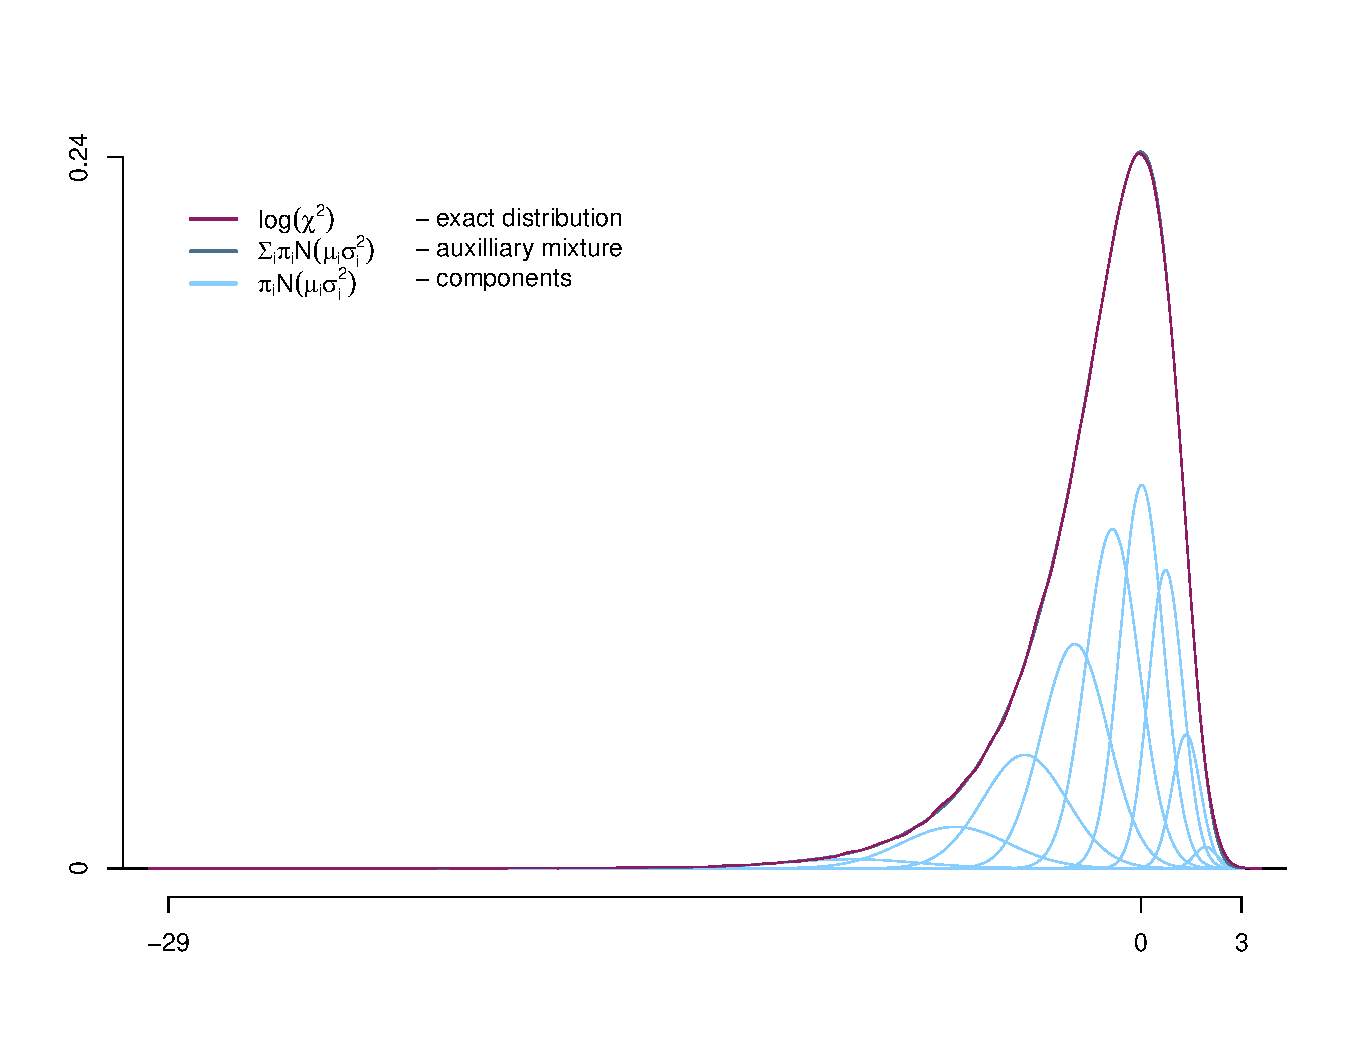
\includegraphics[scale=0.53, trim = 1.5cm 0cm 0cm 1cm]{aux-mix.pdf}
\end{frame}






\begin{frame}{Auxiliary mixture}

\bigskip\textbf{Conditional distribution of $\tilde{\epsilon}_t$}
$$
\tilde{\epsilon}_t|s_t=m \sim\mathcal{N}\left( \mu_{m}, \sigma^2_{m} \right)
$$

\bigskip\textbf{A simple Stochastic Volatility model}
\begin{align}
\tilde{y} &= h + \tilde{\epsilon} \\[1ex]
Hh &= h_0 e_{1.T} + \sigma_v v \\[1ex]
\tilde{\epsilon}|s &\sim \mathcal{N}_T\left( \mu_s, \text{diag}\left(\sigma_s^2\right) \right)\\[1ex]
v &\sim\mathcal{N}_T\left( \mathbf{0}_T, I_T \right)
\end{align}

\small
$$
s = \begin{bmatrix} s_1& \dots & s_T \end{bmatrix}'\quad
\mu_s = \begin{bmatrix} \mu_{s_1}& \dots & \mu_{s_T} \end{bmatrix}'\quad
\sigma_s^2 = \begin{bmatrix} \sigma^2_{s_1}& \dots & \sigma^2_{s_T} \end{bmatrix}'
$$

\end{frame}




{\setbeamercolor{background canvas}{bg=mcxs1}
\begin{frame}

\begin{adjustwidth}{-0.5cm}{0cm}
\FlushLeft
\vspace{8.3cm}\Large
\textbf{{\color{mcxs2}Bayesian estimation} {\color{mcxs5}of SV models}}
\end{adjustwidth}

\end{frame}
}



\begin{frame}{Prior distributions}

\bigskip{\color{mcxs2}Hierarchical prior structure is given by:}
$$
p\left(h,s,h_0,\sigma_v^2\right) = p\left(h|h_0, \sigma_v^2\right)p\left(h_0\right)p\left(\sigma_v^2\right)p\left(s\right)
$$

{\color{mcxs2}Eqs.} (2) {\color{mcxs2}and} (4) {\color{mcxs2}determine a conditional prior distribution of} $h$:
\begin{align*}
p\left(h|h_0, \sigma_v^2\right) &\sim\mathcal{N}_T\left( h_0H^{-1}e_{1.T}, \sigma_v^2(H'H)^{-1} \right)\\
&\propto \det\left(\sigma^2_vI_T\right)^{-
\frac{1}{2}}\exp\left\{ -\frac{1}{2} \frac{1}{\sigma_v^2}(Hh - h_0 e_{1.T})'(Hh - h_0 e_{1.T}) \right\}
\end{align*}
{\color{mcxs2}whereas the marginal prior distributions for} $h_0$, $\sigma_v^2$, {\color{mcxs2}and} $s$ {\color{mcxs2}are:}
\begin{align*}
p(h_0) &= \mathcal{N}(0, \underline{\sigma}_h^2) \\
p\left(\sigma_v^2\right) &= \mathcal{IG}2(\underline{s}, \underline{\nu})\\
p\left(s_t\right) &= \mathcal{M}ultinomial\left(\{m\}_{m=1}^{10}, \{Pr(s_t=m)\}_{m=1}^{10} \right)
\end{align*}

\end{frame}




\begin{frame}{Full-conditional posterior distributions}

\textbf{Full-conditional posterior distribution for $h$}

\smallskip {\color{mcxs2}Equations} (1) {\color{mcxs2}and} (3) {\color{mcxs2}determine the conditional likelihood that is proportional to}
\begin{equation*}
\exp\left\{ -\frac{1}{2} (h - (\tilde{y} - \mu_s))'  \text{diag}\left(\sigma^2_s\right)^{-1} (h - (\tilde{y} - \mu_s)) \right\}
\end{equation*}
{\color{mcxs2}which leads to:}
\begin{align*}
h| y,s,h_0,\sigma_v^2 &\sim\mathcal{N}_T\left(\overline{h},\overline{V}_h  \right)\\
\overline{V}_h &= \left[ \text{diag}\left(  \sigma_s^2\right)^{-1} + \sigma_v^{-2}H'H \right]^{-1} \\
\overline{h} &= \overline{V}_h\left[ \text{diag}\left(  \sigma_s^2\right)^{-1}\left( \tilde{y} - \mu_s \right) + \sigma_v^{-2} h_0e_{1.T}\right]
\end{align*}

\end{frame}






\begin{frame}{Full-conditional posterior distributions}

\textbf{Full-conditional posterior distribution for $s$}

\smallskip {\color{mcxs2}is a multinomial distribution with the probabilities proportional to}
\begin{equation*}
\omega_{m.t} = Pr[s_t=m]p\left(\tilde{y}_t|h_t, s_t=m\right)
\end{equation*}
{\color{mcxs2}for} $m=1,\dots,10$, $p\left(\tilde{y}_t|h_t, s_t=m\right)$ {\color{mcxs2}is based on eqs} (1) \& (3)

\bigskip {\color{mcxs2}For each} $t$ {\color{mcxs2}and} $m$ {\color{mcxs2}obtain} $\omega_{m.t}$ {\color{mcxs2}using parallel computations and compute the probabilities of the multinomial full conditional posterior distribution by }
\begin{equation*}
Pr[s_t=m|\tilde{y}_t, h_t] = \frac{\omega_{m.t}}{\sum_{i=1}^{10}\omega_{i.t}}
\end{equation*}
{\color{mcxs2}Sampling} $s_t$ {\color{mcxs2}independently for each} $t$ {\color{mcxs2}is straightforward}

\end{frame}






\begin{frame}{Full-conditional posterior distributions}

\textbf{Full-conditional posterior distributions for $\sigma_v^2$ and $h_0$}

\smallskip {\color{mcxs2}It is straightforward to show that:}
\begin{align*}
\sigma_v^2| y,s,h,h_0 &\sim\mathcal{IG}2\left(\overline{s},\overline{\nu}  \right)\\
\overline{\nu} &= \underline{\nu} + T \\
\overline{s} &= \underline{s} + (Hh - h_0 e_{1.T})'(Hh - h_0 e_{1.T}) \\[2ex]
h_0| y,s,h,\sigma_v^2 &\sim\mathcal{N}\left(\overline{h}_0,\overline{\sigma}_h^2  \right)\\
\overline{\sigma}_h^2 &= \left( \underline{\sigma}_h^{-2} + \sigma_v^{-2} \right)^{-1} \\
\overline{h}_0 &= \overline{\sigma}_h^2\left( \sigma_v^{-2} e'Hh \right)
\end{align*}

\end{frame}











\begin{frame}{Gibbs sampler}

\bigskip\begin{description}
\item[Initialize] $h^{(0)}$, $s^{(0)}$, and $\sigma_v^{2(0)}$

\bigskip\item[For] $i=1,\dots,S$

\bigskip\smallskip\item[Draw] $h_0^{(i)}\sim\mathcal{N}\left(\overline{h}_0,\overline{\sigma}_h^2  \right)$

\smallskip\item[Draw] $\sigma_v^{2(i)}\sim\mathcal{IG}2\left(\overline{s},\overline{\nu}  \right)$

\smallskip\item[Draw] $s_t^{(i)}\sim\mathcal{M}ultinomial\left(\{m\}_{m=1}^{10}, \{Pr[s_t=m|\tilde{y}_t, h_t^{(i)}]\}_{m=1}^{10} \right)$ \\ for t=1,\dots,T {\color{mcxs2}using inverse transform method}

\smallskip\item[Draw] $h^{(i)}\sim\mathcal{N}_T\left(\overline{h},\overline{V}_h  \right)$ {\color{mcxs2}using precision sampler}

\bigskip\item[Return] {\color{mcxs2}a sample drawn from the posterior distribution:} $$\left\{ h^{(i)}, s^{(i)}, h_0^{(i)}, \sigma_v^{2(i)} \right\}_{i=1}^{S}$$
\end{description}

\end{frame}





\begin{frame}{Simulation smoother}

{\color{mcxs2}The precision matrix of the} $T${\color{mcxs2}-variate normal full-conditional posterior distribution} $\overline{V}_h^{-1}$ {\color{mcxs2}is a tridiagonal matrix.}

\bigskip {\color{mcxs2}Draw random numbers from this distribution using the {\color{purple}simulation smoother} and computer routines for band or tridiagonal matrices.}

\end{frame}


\begin{frame}{Sampling random draws from Multinomial distribution}

\textbf{Inverse transform method}

\centering
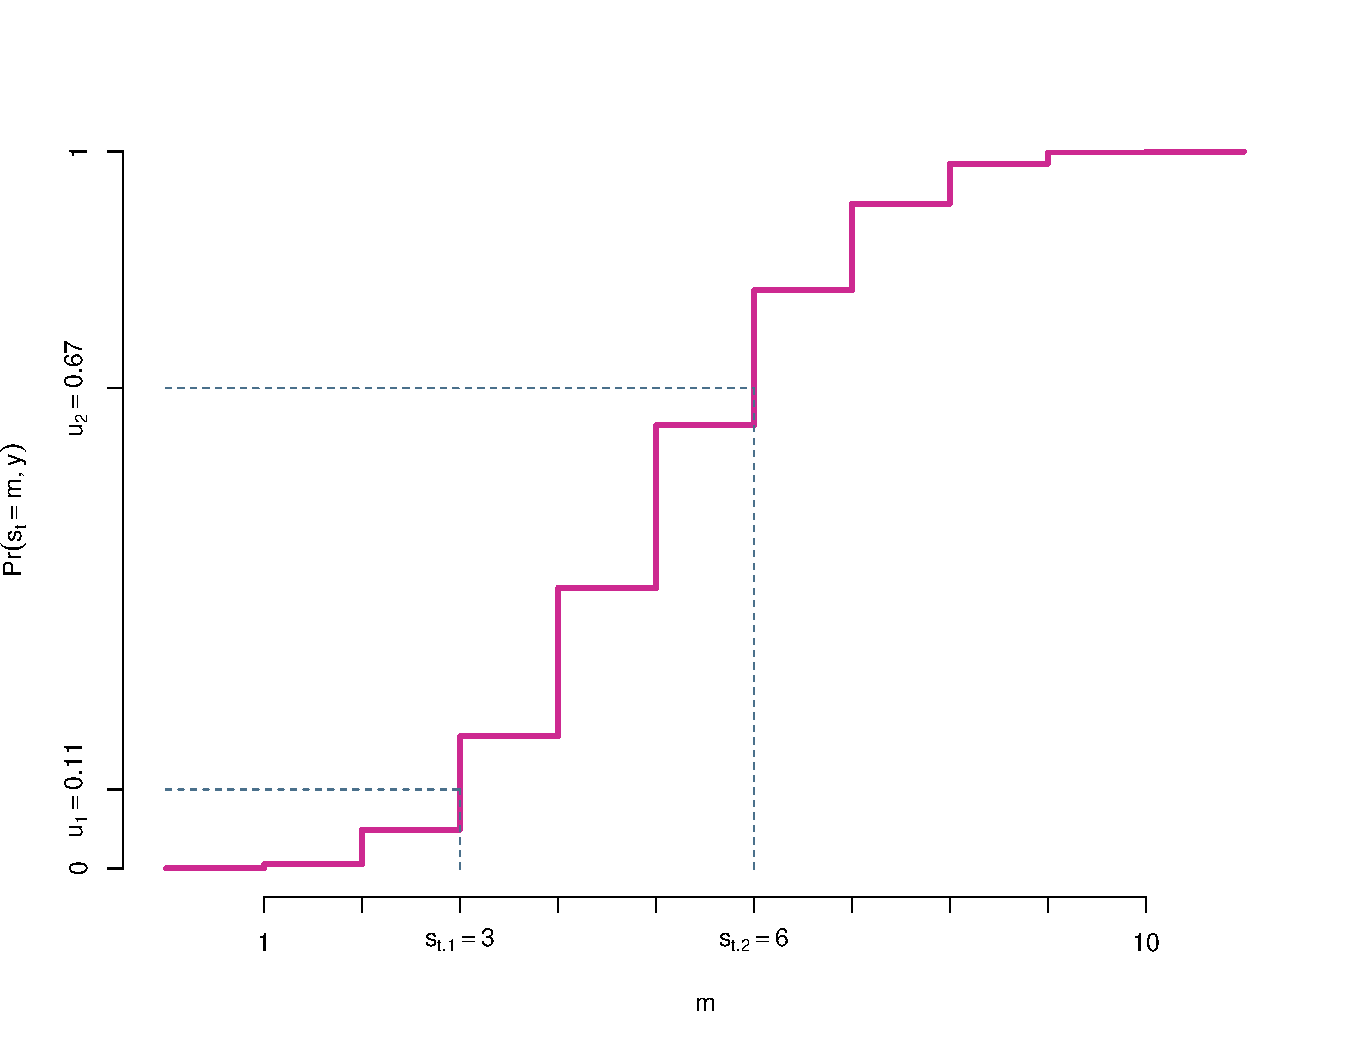
\includegraphics[scale=0.45]{inverse.pdf}
\end{frame}






















{\setbeamercolor{background canvas}{bg=mcxs1}
\begin{frame}

\begin{adjustwidth}{-0.5cm}{0cm}
\FlushLeft
\vspace{8.3cm}\Large
\textbf{{\color{mcxs2}Bayesian estimation} {\color{mcxs5}of the SV--AR models}}
\end{adjustwidth}

\end{frame}
}




\begin{frame}{Bayesian estimation of the SV--AR models}

\bigskip\textbf{An Autoregressive Stochastic Volatility model}
\begin{align*}
y_t &= \exp\left\{\frac{1}{2}h_t\right\} \epsilon_t \\
h_t &= \mu_0  +  \alpha h_{t-1} + \sigma_v v_t \\[1ex]
\epsilon_t &\sim \mathcal{N}\left( 0, 1 \right)\\
v_t &\sim\mathcal{N}\left( 0,1 \right)\\[2ex]
|\alpha|&<1 \quad\text{ -- stationarity condition}
\end{align*}


\end{frame}



\begin{frame}{Bayesian estimation of the SV--AR models}

\bigskip\textbf{An Autoregressive Stochastic Volatility model}
\begin{align*}
\tilde{y} &= h + \tilde{\epsilon} \\[1ex]
H_\alpha h &= \mu_0 \imath_T +  \alpha h_0 e_{1.T} + \sigma_v v \\[1ex]
h &= \mu_0 \imath_T +  \alpha h_{-1} + \sigma_v v \\[1ex]
\tilde{\epsilon}|s &\sim \mathcal{N}_T\left( \mu_s, \text{diag}\left(\sigma_s^2\right) \right)\\[1ex]
v &\sim\mathcal{N}_T\left( \mathbf{0}_T, I_T \right)
\end{align*}

\footnotesize
$$
h_{-1} = \begin{bmatrix} h_0& \dots & h_{T-1} \end{bmatrix}'\quad
\imath_T = \begin{bmatrix} 1& \dots & 1 \end{bmatrix}'\quad
H_\alpha = \begin{bmatrix} 
1 & 0 & \dots & 0 &0\\
-\alpha &1&\dots &0&0\\
\vdots&\vdots&\ddots&\vdots&\vdots&\\
0&0&\dots&1&0\\
0&0&\dots&-\alpha&1\\
\end{bmatrix}
$$

\end{frame}



\begin{frame}{Prior distributions}

\small
\bigskip{\color{mcxs2}Hierarchical prior structure is given by:}
$$
p\left(h,s,h_0,\mu_0, \alpha,\sigma_v^2\right) = p\left(h|\mu_0, \alpha,h_0, \sigma_v^2\right) p\left( \mu_0 \right) p\left(\alpha \right)p\left(h_0\right)p\left(\sigma_v^2\right)p\left(s\right)
$$

{\color{mcxs2}Conditional prior distribution of} $h$:
\begin{align*}
p&\left(h|\mu_0, \alpha,h_0, \sigma_v^2\right) \sim\mathcal{N}_T\left(\mu_0 H_\alpha^{-1}\imath_T+ \alpha h_0H_\alpha^{-1}e_{1.T}, \sigma_v^2(H_\alpha'H_\alpha)^{-1} \right)\\
&\propto \det\left(\sigma^2_vI_T\right)^{-
\frac{1}{2}}\exp\left\{ -\frac{1}{2} \frac{1}{\sigma_v^2}(Hh - \mu_0\imath_T - h_0 e_{1.T})'(Hh - \mu_0\imath_T - h_0 e_{1.T}) \right\}
\end{align*}
{\color{mcxs2}Marginal prior distributions for} $\mu+0, \alpha, h_0,\sigma_v^2$, {\color{mcxs2}and} $s$:
\begin{align*}
p(\mu_0) &= \mathcal{N}(\underline{\mu_0}, \underline{\sigma}_\mu^2) \\
p(\alpha) &= \mathcal{N}(\underline{\alpha}, \underline{\sigma}_\alpha^2)\mathcal{I}(|\alpha|<1)\\
p(h_0) &= \mathcal{N}(0, \underline{\sigma}_h^2) \\
p\left(\sigma_v^2\right) &= \mathcal{IG}2(\underline{s}, \underline{\nu})\\
p\left(s_t\right) &= \mathcal{M}ultinomial\left(\{m\}_{m=1}^{10}, \{Pr(s_t=m)\}_{m=1}^{10} \right)
\end{align*}

\end{frame}




\begin{frame}{Full-conditional posterior distributions}

\textbf{Full-conditional posterior distribution for $h$}

\smallskip {\color{mcxs2}Equations} (1) {\color{mcxs2}and} (3) {\color{mcxs2}determine the conditional likelihood that combined with the conditional prior distribution gives:}
\begin{align*}
h| y,s,\mu_0&,\alpha,h_0,\sigma_v^2 \sim\mathcal{N}_T\left(\overline{h},\overline{V}_h  \right)\\
\overline{V}_h &= \left[ \text{diag}\left(  \sigma_s^2\right)^{-1} + \sigma_v^{-2}H_\alpha'H_\alpha \right]^{-1} \\
\overline{h} &= \overline{V}_h\left[ \text{diag}\left(  \sigma_s^2\right)^{-1}\left( \tilde{y} - \mu_s \right) + \sigma_v^{-2} H_\alpha'\left(\mu_0\imath_T + \alpha h_0e_{1.T}\right)\right]
\end{align*}

\bigskip\textbf{Full-conditional posterior distribution for $s$}

\smallskip {\color{mcxs2}Neither the form of the measurement equation or the multinomial prior distribution changes, therefore, the sampler stays the same. }

\end{frame}






\begin{frame}{Full-conditional posterior distributions}

\textbf{Full-conditional posterior distribution for $\mu_0$}
\begin{align*}
\mu_0| y,h,\alpha,h_0,\sigma_v^2 &\sim\mathcal{N}\left(\overline{\mu}_0,\overline{\sigma}_\mu^2  \right)\\
\overline{\sigma}_\mu^2 &= \left[ \underline\sigma_\mu^{-2} + T\sigma_v^{-2} \right]^{-1} \\
\overline{\mu}_0 &= \overline{\sigma}_\mu^2\left[ \underline{\mu}_0\underline\sigma_\mu^{-2} +  \sigma_v^{-2} \left(H_\alpha h- \alpha h_0e_{1.T}\right)'\imath_T\right]
\end{align*}

\bigskip\textbf{Full-conditional posterior distribution for $\alpha$}
\begin{align*}
\alpha| y,h,\mu_0,h_0,\sigma_v^2 &\sim\mathcal{N}\left(\overline{\alpha},\overline{\sigma}_\alpha^2  \right)\mathcal{I}(|\alpha|<1)\\
\overline{\sigma}_\alpha^2 &= \left[ \underline\sigma_\alpha^{-2} + \sigma_v^{-2}h_{-1}'h_{-1} \right]^{-1} \\
\overline{\alpha} &= \overline{\sigma}_\alpha^2\left[ \underline{\alpha} \underline\sigma_\alpha^{-2} + \sigma_v^{-2} h_{-1}'\left( h- \mu_0\imath_T\right)\right]
\end{align*}

\end{frame}









\begin{frame}{Full-conditional posterior distributions}

\textbf{Full-conditional posterior distribution for $h_0$}
\begin{align*}
h_0| y,h,\alpha,\mu_0,\sigma_v^2 &\sim\mathcal{N}\left(\overline{h}_0,\overline{\sigma}_h^2  \right)\\
\overline{\sigma}_h^2 &= \left[ \underline\sigma_h^{-2} + \alpha^2\sigma_v^{-2} \right]^{-1} \\
\overline{h}_0 &= \overline{\sigma}_h^2\left[ \underline{h}_0\underline\sigma_h^{-2} +  \alpha h_1 \sigma_v^{-2} \right]
\end{align*}

\bigskip\textbf{Full-conditional posterior distribution for $\sigma_v^2$}
\begin{align*}
\sigma_v^2| y,h,&\mu_0,\alpha,h_0 \sim\mathcal{IG}2\left(\overline{s},\overline{\nu}  \right)\\
\overline{s} &= \underline{s} + \left( H_\alpha h-\mu_0\imath_T - \alpha h_0 e_{1.t}\right)'\left( H_\alpha h-\mu_0\imath_T - \alpha h_0 e_{1.t}\right)\\
\overline{\nu} &= \overline{\nu}+T
\end{align*}

\end{frame}







\begin{frame}{Gibbs sampler}

\bigskip\begin{description}
\item[Initialize] $h^{(0)}$, $s^{(0)}$, $\mu_0^{(0)}$, $\alpha^{(0)}$, and $\sigma_v^{2(0)}$

\bigskip\item[For] $i=1,\dots,S$

\bigskip\smallskip\item[Draw] $h_0^{(i)}\sim\mathcal{N}\left(\overline{h}_0,\overline{\sigma}_h^2  \right)$

\smallskip\item[Draw] $\sigma_v^{2(i)}\sim\mathcal{IG}2\left(\overline{s},\overline{\nu}  \right)$


\smallskip\smallskip\item[Draw] $\mu_0^{(i)}\sim\mathcal{N}\left(\overline{\mu}_0,\overline{\sigma}_\mu^2  \right)$

\smallskip\item[Draw] $\alpha^{(i)}\sim\mathcal{N}\left(\overline{\alpha},\overline{\sigma}_\alpha^2  \right)$


\smallskip\item[Draw] $s_t^{(i)}\sim\mathcal{M}ultinomial\left(\{m\}_{m=1}^{10}, \{Pr[s_t=m|\tilde{y}_t, h_t^{(i)}]\}_{m=1}^{10} \right)$\\ for $t=1,\dots,T$ {\color{mcxs2}using inverse transform method}

\smallskip\item[Draw] $h^{(i)}\sim\mathcal{N}_T\left(\overline{h},\overline{V}_h  \right)$ {\color{mcxs2}using precision sampler}

\bigskip\item[Return] {\color{mcxs2}a sample drawn from the posterior distribution:} $$\left\{ h^{(i)}, s^{(i)}, \mu_0^{(i)}, \alpha^{(i)}, h_0^{(i)}, \sigma_v^{2(i)} \right\}_{i=1}^{S}$$
\end{description}

\end{frame}










{\setbeamercolor{background canvas}{bg=mcxs1}
\begin{frame}

\begin{adjustwidth}{-0.5cm}{0cm}
\FlushLeft
\vspace{8.3cm}\Large
\textbf{{\color{mcxs2}Introduction to} {\color{mcxs5}heteroskedastic models}}
\end{adjustwidth}

\end{frame}
}




\begin{frame}{Introduction to heteroskedastic models}

\bigskip\textbf{A linear regression with Stochastic Volatility}
\begin{align*}
Y & = X\beta +E\\
E\mid X &\sim\mathcal{N}_T\left( \mathbf{0}_T, \text{diag}\left( \sigma^2\right)\right)\\[2ex]
\sigma^2 &= \left( \exp\{h_1\}, \dots, \exp\{h_T\} \right)\\
h_t &\text{ -- follows a Stochastic Volatility process}\\[1ex]
\beta &\sim\mathcal{N}\left( \underline\beta, \underline{V}_\beta\right)
\end{align*}

\bigskip\textbf{A model with conditional heteroskedasticity}
\begin{itemize}[label=$\blacktriangleright$]
\item Improves the precision of the estimation of $\beta$
\item Improves the in-sample fit of the model
\item Greatly improves the forecasting performance of the model
\end{itemize}

\end{frame}




\begin{frame}{Introduction to heteroskedastic models}

\bigskip\textbf{Full conditional posterior distribution of $\beta$}
\begin{align*}
\beta \mid Y,X,h &\sim\mathcal{N}\left( \overline\beta, \overline{V}_\beta\right)\\[2ex]
\overline{V}_\beta & = \left[ \underline{V}_\beta^{-1} + X'\text{diag}\left(\sigma^2\right)^{-1}X\right]^{-1}\\
\overline\beta &= \overline{V}_\beta \left[ \underline{V}_\beta^{-1}\underline\beta + X'\text{diag}\left(\sigma^2\right)^{-1}Y\right]
\end{align*}

\bigskip Conditionally on $h$ the remaining model parameters can be sampled from their respective full conditional posterior distributions that take into account the conditional variances of the error term
\end{frame}












{\setbeamercolor{background canvas}{bg=mcxs1}
\begin{frame}{Bayesian estimation of SV models}

\begin{description}
\item[\color{mcxs5}An efficient and computationally fast] {\color{mcxs3}method of estimating SV models is Bayesian Gibbs sampler}
\bigskip\item[\color{mcxs5}Dedicated computational techniques] {\color{mcxs3}include}
	\begin{description}
	\item[\color{mcxs5}auxiliary mixture]
	\item[\color{mcxs5}simulation smoother]
	\item[\color{mcxs5}operations on tridiagonal matrices]
	\item[\color{mcxs5}inverse transform method]
	\end{description}

\bigskip\item[\color{mcxs5}The algorithm] {\color{mcxs3}presented in this lecture is applicable to}
	\begin{description}
	\item[\color{mcxs5}univariate models] {\color{mcxs3}with SV conditional heteroskedasticity}
	\item[\color{mcxs5}multivariate models] {\color{mcxs3}with independent SV processes}
	\end{description}

\bigskip\item[\color{mcxs5}Adapt] {\color{mcxs3}your Gibbs sampler to use function} \texttt{\color{mcxs5}SV.Gibbs.iteration} {\color{mcxs3}from file} \texttt{\color{mcxs5}00 SV codes.R}
\end{description}

\end{frame}
}

\end{document} 